\documentclass[output=paper]{langsci/langscibook} 
\author{Isabelle Udry\affiliation{University of Fribourg, Institut de Plurilinguisme; Zurich University of Teacher Education} and Raphael Berthele\affiliation{University of Fribourg, Institut de Plurilinguisme}}
\title{Introduction to the volume}
\abstract{This introduction outlines the main focus and features of the project Language Aptitude at Primary School (LAPS). We begin with the rationale for the study and some clarification on terminology used throughout the book. Next, we discuss key concepts underlying language learning ability and early foreign language tuition. Finally, we provide an overview of the study design and the contents of the volume.
}
\IfFileExists{../localcommands.tex}{
  \addbibresource{localbibliography.bib}
  % add all extra packages you need to load to this file

\usepackage{tabularx,multicol}
\usepackage{url}
\urlstyle{same}

\usepackage{listings}
\lstset{basicstyle=\ttfamily,tabsize=2,breaklines=true}

%\usepackage{langsci-optional}
\usepackage{langsci-lgr}
\usepackage{langsci-gb4e}
\usepackage{langsci-optional}

\usepackage{enumitem}
\usepackage[group-digits=false, detect-weight=true]{siunitx}

\usepackage{todonotes}

  \newcommand*{\orcid}{}
 
  %% hyphenation points for line breaks
%% Normally, automatic hyphenation in LaTeX is very good
%% If a word is mis-hyphenated, add it to this file
%%
%% add information to TeX file before \begin{document} with:
%% %% hyphenation points for line breaks
%% Normally, automatic hyphenation in LaTeX is very good
%% If a word is mis-hyphenated, add it to this file
%%
%% add information to TeX file before \begin{document} with:
%% %% hyphenation points for line breaks
%% Normally, automatic hyphenation in LaTeX is very good
%% If a word is mis-hyphenated, add it to this file
%%
%% add information to TeX file before \begin{document} with:
%% \include{localhyphenation}
\hyphenation{
affri-ca-te
affri-ca-tes 
Soa-res
scru-ti-ny
me-ta-cog-ni-tion
}

\hyphenation{
affri-ca-te
affri-ca-tes 
Soa-res
scru-ti-ny
me-ta-cog-ni-tion
}

\hyphenation{
affri-ca-te
affri-ca-tes 
Soa-res
scru-ti-ny
me-ta-cog-ni-tion
}
 
  \togglepaper[1]%%chapternumber
}{}

\begin{document}
\maketitle 

\section{About this volume}

Since the beginning of the new millennium, early foreign language teaching and learning has seen important changes, namely the lowering of the starting age for language classes across Europe and the mandatory introduction of two foreign languages at primary schools in Switzerland, where this study took place. These developments led to debate and even controversy that required empirical evidence to underpin the arguments. It was against this backdrop that the idea for the project \textit{Language Aptitude at Primary School} (LAPS) emerged. We assessed the impact of a set of individual difference (ID) variables and environmental factors on young learners’ developing foreign language proficiency over a period of two academic years. Our aim was to provide new insights into what shapes 10--12-year-old children’s foreign language learning in minimal input settings with 2--3 weekly lessons. Particular attention was paid to language aptitude which has been extensively researched with adults but has only recently sparked scholarly interest in relation to young learners (for a discusson see Chapter 1, §2.2). We hope that the findings presented in this volume will be useful to both educators and researchers. 

\subsection{Reader’s guide}

This introduction contains all information needed to follow the empirical chapters. In addition, two introductory chapters provide more details on the theoretical framework of the LAPS project (Chapter 1) and the study design (Chapter 2). Readers are invited to read Chapters 1 and 2 before embarking on the rest of the volume or consult them as questions arise during reading. Chapters 3 to 10 cover different aspects of the LAPS project (outlined in \sectref{sec:intro:5} of this chapter) and are conceived as independent texts with the main information being summarized in the abstracts and methodology sections of each chapter. For the sake of replicability, supplementary material, including datasets and R scripts, have been made available online: \url{https://osf.io/hstv7/}.

\subsection{Terminology}

With four official languages (German, French, Italian, and Rumantsch) and a variety of heritage languages, Switzerland’s linguistic landscape is certainly diverse. This calls for some introductory remarks on the use of terminology in this volume. 

L1 refers to the first language of the children. School language German (or German as a school language) describes the language of literacy or language of instruction in the LAPS region. Second language (L2) and third language (L3) designate the foreign languages taught at primary school in order of introduction: L2 refers to the first foreign language and L3 to the second foreign language introduced as part of the mandatory Swiss curriculum. 

We are aware that on entering primary school, many children in Switzerland already have several languages in their repertoire, either because they are heritage language speakers, because they speak a Swiss German (Alemannic) dialect at home, or because of family ties with other linguistic regions of the country (see \citealt{Berthele2020} for a discussion of these difficulties in counting languages in the multilingual repertoire). To these children, foreign languages taught at school are actually their fourth or fifth language and German may not be their L1. Nevertheless, we adhere to using L2/L3 for instructed language teaching and learning, particularly for ease of reading.

As will be outlined in \sectref{sec:intro:4.2}, the project consists of two subprojects, LAPS I and LAPS II. Throughout the volume, we will use the term LAPS when referring to the project in general, and LAPS I or LAPS II when talking about the specific subprojects.

\section{A talent for language learning} 

Being a successful language learner often comes with a great deal of recognition. Whether it be the hyper-polyglot conversing fluently in many languages (e.g. \citealt{Erard2012}), or the person who has picked up a native-like accent in a language different from their first (\citealt{FlegeMackay2011}; \citealt{ChristinerReiterer2015}), both are likely to encounter admiration for their achievements, and most certainly the question: “How do you do it?” 

The notion of a talent for language learning was first theorized in the United States by John B. Carroll during the 1950s and 60s. The main reason for studying the characteristics of successful language learners was to provide government institutions with tools to select promising candidates for state-funded language courses. To this aim, \citet{Carroll1964} administered a range of tests deemed to capture key abilities for language learning to members of staff at the US Army. From the results, he derived four language-related factors he subsumed under the term \textit{language aptitude:} 

\begin{enumerate}
\item \textit{phonetic coding} (the ability to store, identify, and remember auditory phonetic material), 
\item \textit{grammatical sensitivity} (the ability to recognize the grammatical functions of elements in clauses), 
\item \textit{inductive language learning} (the ability to discover grammatical rules independently), and 
\item \textit{rote memory} (the ability to memorize new words rapidly and then retrieve them from memory). 
\end{enumerate}

Based on these components, \citet{CarrollSapon1959} developed the Modern Language Aptitude Test (MLAT) which became widely used for selection and research purposes. However, the view on language aptitude as a predetermined attribute that could regulate access to language education soon came under scrutiny by educational stakeholders and scholars. Also, new (communicative) approaches to language teaching were considered to transform learning in a way that neutralized individual differences in language learning aptitude \citep[72]{Skehan2002}. Concomitant with dominant views on individuals and societies in academia in the last decades of the 20\textsuperscript{th} century, the idea that people differ in their ability to think and learn beyond what can be explained by social differences had become very unfashionable, to say the least. As argued in \citet[28]{Pinker2003} the idea of the “ghost in the machine”, that is that humans are malleable and can be made better (or worse) by pedagogy became the “watchword of social science”.

\subsection{New perspectives} 

While the discomfort with the Carrollian aptitude construct led to a marked decrease in scientific activity for several decades, language aptitude never entirely disappeared from the research agenda. Recent scholarly interest has moved away from merely forecasting L2 achievement for selective purposes. Instead, relating language aptitude to SLA theories has become a main focus that has drawn attention from disciplines beyond applied linguistics, such as educational and cognitive psychology, or the neurosciences \citep{WenEtAl2019Researching}. 

Extending on the cognitive-linguistic focus reflected in the early stages of aptitude research, the ability to learn and communicate in a foreign language is currently regarded as being governed by a multitude of factors which can be grouped into three categories \citep{Reiterer2009}: \textit{biological} (e.g., DNA, sex, hormones), \textit{linguistic\slash socio-cultural} (e.g., quality and quantity of input, language attitudes, typological distance/closeness between languages), and \textit{psycho(bio)logical factors} (e.g., motivation, verbal intelligence, and language aptitude as defined in the previous paragraphs). A broad view that subsumes biological, language-related, cognitive, and affective factors that are studied from multiple scientific perspectives, holds promising prospects for advancing theories of foreign language learning and SLA. Recently, a number of innovative research projects have been conducted, the results of which can be consulted for instance in volumes by \citet{Reiterer2019} or \citet{WenEtAl2019}. 

\subsection{Nature and nurture}

Reviewing various studies that defined language aptitude as the ability to deal with language phonetically, grammatically, lexically or pragmatically, \citet{Reiterer2019} concludes that these skills and abilities are normally distributed in the population. With reference to the bell-shaped curve, this means that a small group of about 15\% will achieve very high, possibly near-native proficiency, while another 15\% will retain very little of a foreign language. The remaining majority of about 70\% will reach average skill levels. Language learning ability is therefore present in all individuals to varying degrees and the question of language talent cannot be answered by a simple yes or no statement.

Normally distributed characteristics, such as height, weight or intelligence, have been linked to some biological underpinning \citep{Reiterer2019}. There has been ongoing debate in psycholinguistics on the extent to which language learning and variations in achievement are genetically wired. Recent large-scale adoption and twin studies provide evidence that a considerable proportion of success in second and foreign language learning can be explained by hereditary factors. According to some studies, the genetic-makeup explains 50\% or more of the variance in various aspects of human cognition (\citealt{DaleEtAl2010}; \citealt{Stromswold2001}; \citealt{RimfeldEtAl2015}). This would still leave up to half of the variance to be attributed to factors other than genes, an observation that may alleviate some of the early apprehensions about language aptitude being fixed at birth and paving the way for inegalitarian practices in education. It also ties in with the question whether language learning ability could be influenced or even be trained by providing specific educational conditions. 

In sum, key questions regarding language learning ability are a) the impact of individual predispositions (including aptitude, general learning abilities, and motivation) and external influences (such as socioeconomic status, teaching conditions, quantity and quality of input) on language competence; b) the extent to which these influencing factors can be changed by experience or training; and c) the relationship between individual predispositions, especially domain specific and general cognitive abilities.  

\section{Children and foreign language learning in Europe …}

The European Union (EU) considers linguistic and cultural diversity as one of its main assets worth promoting. Based on recommendations made by the \citet[19]{BarcelonaEuropeanCouncil2002}, the general aim for EU citizens is now mastery of basic skills in at least two foreign languages. An early start to language learning at school has been declared a key strategy in pursuing this ambitious objective \citep{EuropeanCommission2004}. This has led to the starting age for foreign language classes being lowered across Europe in recent years. According to the 2012 Euridyce\slash Eurostat survey conducted in 32 European countries, the usual starting age in 2009/10 was between 6 and 9 years. 78\% of all children attending primary school in 2009/10 were learning a foreign language, in most cases English \citep[10f]{Eurostat2012}.

The introduction of early language teaching in Europe and beyond has not gone without some major challenges, particularly in relation to developing appropriate educational frameworks. Main difficulties emerged in drafting generalizable policies underpinned by sound assumptions about children’s learning \citep{Johnstone2009} and implementing these policies with adequate resources, such as age-appropriate teaching models and materials, or well-prepared teachers (for a discussion see \citealt{GartonEtAl2011}). Early instructed language learning also led to increased research activity, with teaching principles and age-related questions being explored in several large-scale studies, most notably by \citet{EdelenbosEtAl2006}, \citet{Muñoz2006}, \citet{NikolovCsapó2010}, \citet{Enever2011}, \citet{GartonEtAl2011}, \citet{Pfenninger2016}, \citet{JaekelEtAl2017}, and \citet{BaumertEtAl2020}.

\section{… and Switzerland}

The European trend has no doubt influenced policy development in Switzerland. Because of its multilingual context with four official languages, foreign language learning has a longstanding tradition in the country. As early as 1975, the Swiss government’s recommendation for teaching one foreign language at primary school was being implemented throughout the country (for more details on the history of foreign language teaching in Switzerland see \citealt{GiudiciGrizelj2016}). In the early 2000s, a new national strategy prescribed the introduction of even two foreign languages at primary school \citep{EDK2004}, one at age 9, the second at age 11. At least one of them had to be a national language, the other could be English. Owing to the federal system, the cantons were free to choose how they would put the strategy into place, i.e. which two languages they wanted to introduce to children in what order. This led to considerable debate, as some cantons opted to start with English, rather than a national language. This choice was seen as a threat to national cohesion by some citizens, especially speakers of the minority national languages French, Italian and Rumantsch \citep{Stotz2006}.

Moreover, concerns were expressed about some learner groups being overwhelmed by the demands of studying two foreign languages. However, while heavily debated, it was difficult to substantiate these fears with empirical evidence\footnote{The \citet{SchweizerischeAkademiederGeisteswissenschaften2015} published an overview on the arguments used in the Swiss debate.}. In the end, and as for many aspects of educational planning, the cantons were left to handle dispensation from foreign language classes as they saw fit.

\section{The project Language Aptitude at Primary School (LAPS)}

The project comprises two parts, LAPS I and LAPS II, which took place between spring 2017 and spring 2019. Samples and data collection are summarized in Tables 1 and 2. The children came from Swiss public schools, i.e. non-selective state-funded schools that teach all children living in their catchment area. Participants in both projects attended grades 4 and 5 (10 and 11 years) at the beginning of the study and were learning an L2 and L3 with 2--3 weekly lessons per language as part of the mandatory curriculum. At the beginning of the study, all participants completed a test battery assessing a great number of individual difference (ID) variables (see \figref{fig:intro:1}). The results were related to their L2 and/or L3 proficiency. In the first part of the project (LAPS I), we considered L2 French and L3 English proficiency cross-sectionally ($n=174$). In the second subproject (LAPS II, $n=637$\footnote{This number pertains to the total of individuals participating in at least one of three data collections of LAPS II. Due to children leaving or joining the project, this number differs from the total for each data collection indicated in \tabref{tab:intro:2}.}), we recorded children’s development of L2 English proficiency over two academic years (1.5 years).

\subsection{Individual difference (ID) variables and environmental factors}

Starting from the assumption that learning in general is influenced by a multitude of individual and contextual factors, we adopted a largely psycholinguistic perspective for this study with reference to the literature on individual differences (ID) in foreign language learning. We also included variables pertaining to the children’s social background as previous research has consistently found them to be related to learning. A main objective of the project was to better understand how language aptitude in the Carrolian sense is implicated in child learning, an issue that has received little attention in research so far. Independent variables selected for the study fall into four categories:

\begin{enumerate}
\item Language aptitude 

\begin{itemize}
\item grammatical sensitivity
\item inductive learning\footnote{Based on a definition by \citet{Skehan1998}, grammatical sensitivity and inductive ability can be subsumed as language analytic ability.}
\item phonetic coding ability
\item rote memory
\end{itemize}

\item General cognitive abilities or general learning abilities
\begin{itemize}
\item intelligence
\item working memory
\item creativity
\item cognitive style (field independence)
\end{itemize}

\item Affective Dispositions

\begin{itemize}
\item L2/L3 motivation
\item foreign language learning anxiety
\item L2/L3 self-concepts
\item dedication
\item perceived support from teachers and parents
\item locus of control
\end{itemize}

\item Environmental factors or background variables

\begin{itemize}
\item socioeconomic status (SES)
\item language background
\item teaching paradigm 
\end{itemize}
\end{enumerate}

\figref{fig:intro:1} shows the structure of the independent variables. Environmental factors are assumed to be overarching, as it is difficult for the individual to change them. Individual predispositions (or ID variables) are nested within these environmental factors. Based on the literature, it is assumed that there is interaction between social status, linguistic background or approaches to teaching, and the affective dispositions, such as motivation to learn foreign languages and anxiety. The dynamicity between these categories is indicated by the dotted line (and the arrow pointing from environmental to affective). Also, some fluidity between language aptitude and general cognitive variables is expected, most notably for memory functions (see Chapter 1, §2.3 for a discussion). Rote memory which stands for the ability to rapidly map meaning to sound/word form, is part of the aptitude construct. Recently however, some researchers have suggested extending on this component with a more current definition of memory, based on the working memory model by \citet{BaddeleyHitch1974}. 

\begin{figure}
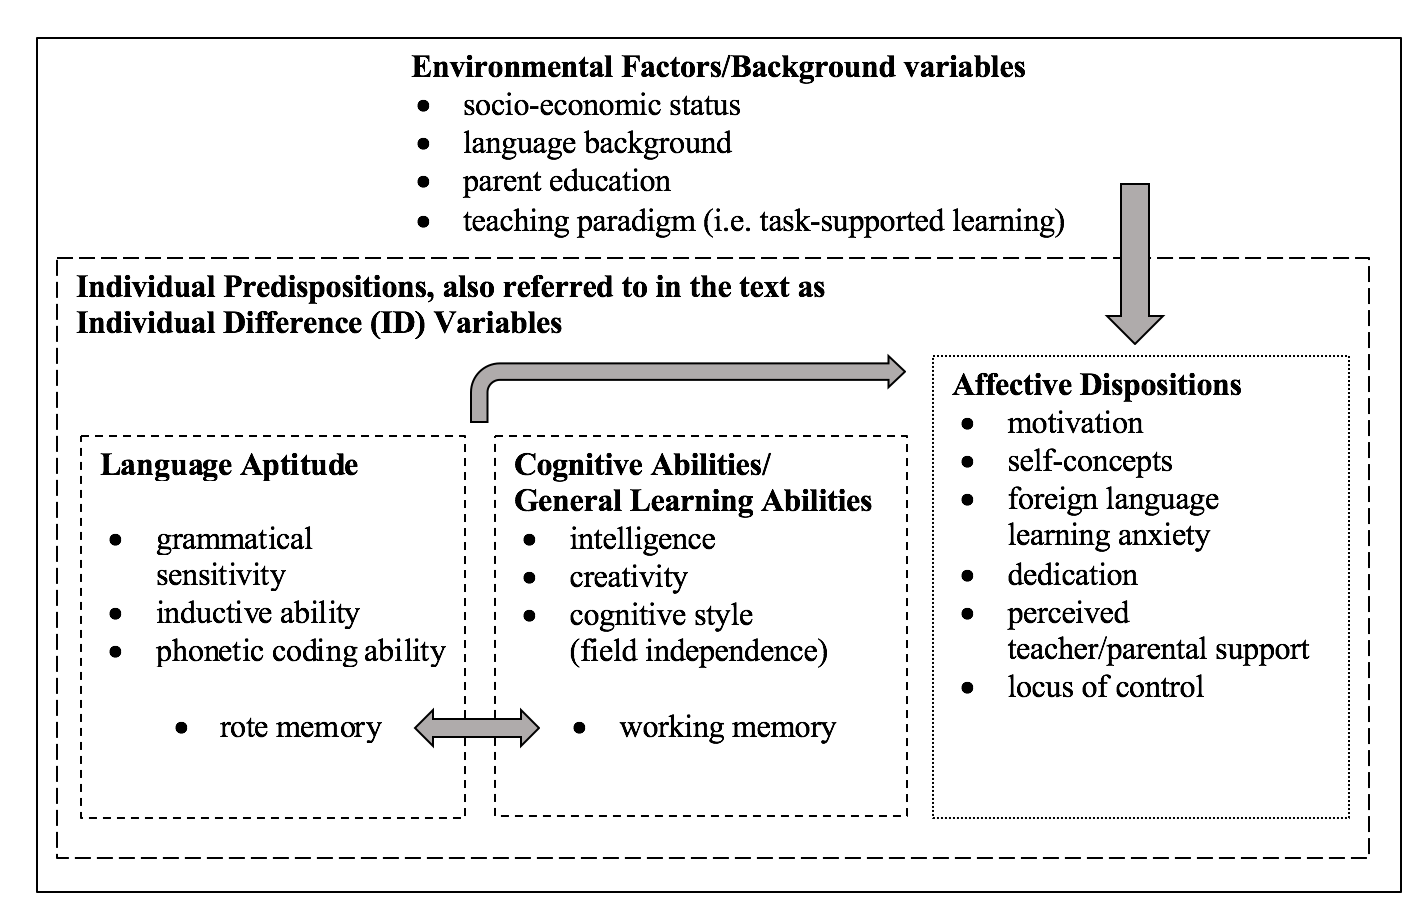
\includegraphics[width=\textwidth]{figures/intro-fig1.png}
\caption{Structure of independent variables. Dotted lines indicate that the clear-cut categorization can be questioned. Arrows show expected direction of interaction.\label{fig:intro:1}}
\end{figure}

\subsection{Research questions}\label{sec:intro:4.2}

The following research questions were addressed in the LAPS project:

\begin{itemize}
\item What ID variables are predictive of children’s L2 proficiency and to what extent?
\item What is the relationship between these variables, especially aptitude and general learning abilities?
\item What developmental patterns can be observed in L1 and L2 proficiency, aptitude, and motivation?
\item How do environmental factors affect children’s L2 learning, (most notably SES, living close to a native speaking community)?
\end{itemize}


\subsection{Design and procedures}
\subsubsection{LAPS I}

The first subproject was conducted with 4\textsuperscript{th} and 5\textsuperscript{th} graders from 10 classes located at the border with French-speaking Switzerland. Children’s school language was German, they learnt L2 French (starting in 3\textsuperscript{rd} grade, at 9 years old) and L3 English (starting in 5\textsuperscript{th} grade, at 11 years old). Two data collections took place: T1 in spring 2017 ($n=174$, mean age 11.1) and T2 in spring 2018 ($n=158$, mean age 12.1).

In LAPS I, the test battery was piloted and some changes were added for LAPS II (see Chapter 2, §3.1 for details). A second data collection T2 was included for two reasons: 1) to investigate the longitudinal development of affective dispositions. We wanted to find out how living close to native speakers of French would be reflected in the children’s motivation to learn French and English over time (Chapter 7); 2) to understand the relationships between L2 and L3 skills (published in \citealt{BertheleUdry2019}). To address these aims, the questionnaire on affective dispositions was re-administered and a measure of L3 English proficiency was added at T2. T2 had not been part of the overall design and was added as a follow-up project in the context of research training for students in the Fribourg multilingualism Master’s program.

\begin{table}\footnotesize
\caption{\label{tab:intro:1}Summary main information LAPS I}
\begin{tabularx}{\textwidth}{lp{\widthof{mean age: 12.1}}>{\hangindent=2ex}QQ}

\lsptoprule

{Date} & {Participants} & {Independent variables} & {Language proficiency}\\\midrule
{T1 spring 2017} & {4\textsuperscript{th}\slash 5\textsuperscript{th} grade}

{$n=174$}

{mean age: 11.1} & Entire test battery:\newline aptitude\newline general cognitive abilities\newline affective ID variables\newline background variables & {L2 French}

{School language German}\\\tablevspace
{T2 spring 2018} & {5\textsuperscript{th}\slash 6\textsuperscript{th} grade} 

{$n=158$}

{mean age: 12.1} & {L2/L3 affective ID variables} & {L3 English}\\
\lspbottomrule
\end{tabularx}
\end{table}

\subsubsection{LAPS II}

32 classes from the Eastern part of Switzerland participated in LAPS II for a period of two academic years (1.5 years in total). At the beginning of the study, the children were either in 4\textsuperscript{th} or 5\textsuperscript{th} grade (mean age 10.5), at the end of the study in 5\textsuperscript{th} or 6\textsuperscript{th} grade (12.1 years old). These children’s school language was German, they learnt L2 English (starting in 2\textsuperscript{nd} grade, at the age of 8) and L3 French (starting in 5\textsuperscript{th} grade, at the age of 11).

LAPS II was longitudinal so we could trace the development of a) language proficiency in L2 English, b) school language German, c) language aptitude (grammatical sensitivity and inductive ability), d) affective dispositions. 

Data was collected three times in the same classes: At T1 (autumn 2017), we administered the entire test battery with all ID variables, L2 proficiency, and proficiency in school language German to all children. At T2 (spring 2018) and T3 (spring 2019), five measures were re-administered to the same participants to monitor longitudinal development: 1) L2 English proficiency, 2) school language German proficiency, 3) language aptitude (grammatical sensitivity) 4) language aptitude (inductive ability), 5) L2/L3 motivation questionnaire. 

\begin{table}\footnotesize
\caption{Summary main information LAPS II\label{tab:intro:2}}
\begin{tabularx}{\textwidth}{lp{\widthof{mean age: 12.1}}>{\hangindent=2ex}QQ}
\lsptoprule

{Date} & {Participants} & {Independent variables} & {Language proficiency}\\\midrule
{T1 autumn 2017} & {4\textsuperscript{th}\slash 5\textsuperscript{th} grade}

{$n=615$}

{mean age: 10.5} & entire test battery:\newline aptitude\newline general cognitive abilities\newline affective ID variables\newline background variables & {L2 English}

{school language German proficiency}\\\tablevspace
{T2 spring 2018} & {4\textsuperscript{th}\slash 5\textsuperscript{th} grade}

{$n=578$}

{mean age: 11.1} & aptitude:\newline grammatical sensitivity\newline inductive ability & {L2 English}

{school language German proficiency}\\
                 & & L2/L3 affective ID variables & \\\tablevspace
{T3 spring 2019} & {5\textsuperscript{th}\slash 6\textsuperscript{th} grade}

{$n=566$}

{mean age: 12.1} & aptitude:\newline grammatical sensitivity\newline inductive ability & {L2 English}

{school language German proficiency}\\
                 & & L2/L3 affective ID variables & \\
\lspbottomrule
\end{tabularx}
\end{table} 

\section{Findings}\label{sec:intro:5}

The results of the project are presented in Chapters 3 to 10. Chapter 3 discusses the various dimensions of the ID variables assessed in the test battery and their impact on L2 learning by primary school children. Chapter 4 deals with the predictive power of these ID variables for the participants’ L2 proficiency.

The second part of the volume is devoted to more specific issues of the LAPS project. Chapter 5 examines the impact of socioeconomic factors, Chapter 6 looks into a less researched variable, i.e. creativity, within the context of task-based language learning, and Chapter 7 is dedicated to the role of motivation for L2/L3 learning at primary school. Chapters 8 to 10 address developmental patterns associated with ID variables over two academic years. Chapter 8 investigates changes in motivation, Chapter 9 covers the relationship between skills in the language of instruction (German) and L2 English proficiency, and Chapter 10 explores the extent to which language aptitude, i.e. its language analytic subcomponent, remains stable over time.

We hope that this volume will incite discussion on early instructed language learning and encourage further scientific activity related to child L2/L3 learning which we deem to be a viable research topic.

\section*{Acknowledgments}

The LAPS project has been funded by the Research Centre on Multilingualism at the University of Fribourg and Teacher Training College of Fribourg, Switzerland. 

Many people have contributed to the successful running of the project. Most importantly, we thank the teachers and pupils who remained committed to our project for so long. It could not have happened without them. Many thanks to Charles W. Stansfield for letting us translate and adapt forms of the MLAT-E and PLAB tests. Our thanks go to a panel of experts who have guided us with their invaluable advice throughout the entire endeavour: Esther Geva, Joachim Grabowski, Susanne Reiterer. We are grateful to Amelia Lambelet for her contribution to LAPS I. To Peter Lenz for generously sharing his expertise and assisting us in selecting a suitable English measure. Raphael Marguet from the Atelier Multimédia at the PH Fribourg for his support in recording test instructions. Isabelle Affolter for her care in proofreading parts of the manuscript. We thank our fieldworkers for their help with data collection and processing. Their dedication has greatly added to the quality of the project: Josef Adler, Thomas Aeppli, Nael Ackermann, Alessandra Dedei, Kinga Dobrowolska, Paola Gagliardi, Noemi Gloor, Alessandra Gregori, Laura Hodel, Rachel Howkins, Patricia Isler, Alexandra Jaszkowski, Jasmin Koch, Luca Krenger, Bente Lowin Kropf, Nina Müller, Heike Reimann, Pauline Robert-Charrue, Maja Schärer, Sarah Singh, Fabio Soares, Laura Sopa, Tanja Zepf, Catarina Zweidler. 

{\sloppy\printbibliography[heading=subbibliography,notkeyword=this]}
\end{document}
